\documentclass{article}

% if you need to pass options to natbib, use, e.g.:
%     \PassOptionsToPackage{numbers, compress}{natbib}
% before loading neurips_2021

% ready for submission
\usepackage[final]{neurips_2021}
% to compile a preprint version, e.g., for submission to arXiv, add add the
% [preprint] option:
%     \usepackage[preprint]{neurips_2021}

% to compile a camera-ready version, add the [final] option, e.g.:
%     \usepackage[final]{neurips_2021}

% to avoid loading the natbib package, add option nonatbib:
%    \usepackage[nonatbib]{neurips_2021}

\usepackage[utf8]{inputenc} % allow utf-8 input
\usepackage[T1]{fontenc}    % use 8-bit T1 fonts
\usepackage{hyperref}       % hyperlinks
\usepackage{url}            % simple URL typesetting
\usepackage{booktabs}       % professional-quality tables
\usepackage{amsfonts}       % blackboard math symbols
\usepackage{nicefrac}       % compact symbols for 1/2, etc.
\usepackage{microtype}      % microtypography
\usepackage{xcolor}         % colors
\usepackage{graphicx}       % images

\title{Milestone 1 8420}

% The \author macro works with any number of authors. There are two commands
% used to separate the names and addresses of multiple authors: \And and \AND.
%
% Using \And between authors leaves it to LaTeX to determine where to break the
% lines. Using \AND forces a line break at that point. So, if LaTeX puts 3 of 4
% authors names on the first line, and the last on the second line, try using
% \AND instead of \And before the third author name.

\author{%
	Will Sherrer \\
	Clemson University\\
	wsherre@g.clemson.edu \\
	\And Ashton Sobeck \\
	Clemson University\\
	asobeck@g.clemson.edu
}





\begin{document}
\maketitle
%\section{Submission of papers to NeurIPS 2021}
\section{Introduction}

CNN's take images and use filters to classify them into different categories. While training a CNN is a novel concept today, tweaking the parameters and structure of a CNN is a problem that depends on different variables. What we want to focus on is also the data that is fed into a CNN. Since these networks are so powerful we want to test the limit of their abilities. Image recognition systems have been in place for a while and will only get better. As the amount of images on the internet and devices will only grow storing them could pose as a challenge. With this project we hope to see if training CNN's on compressed images can be as effective as normal ones. This could help reduce data if compressed images can be regenerated, and classified as well as uncompressed ones. 

\section{Method}

We are reducing these images via PCA. We plan to train 2 models with the regular dataset, and the CIFAR-10 dataset reduced by 20\%, 40\%, 60\%, and 80\%. We will compare the Training and Testing Loss and Accuracy. 

\section{Current Progress}

Currently we have designed 2 models that are trainable and testable. These models are both CNN's that will be trained in the CIFAR dataset. We wanted to do 1 smaller model and 1 larger model to see if the added parameters help identify images.
\begin{figure}
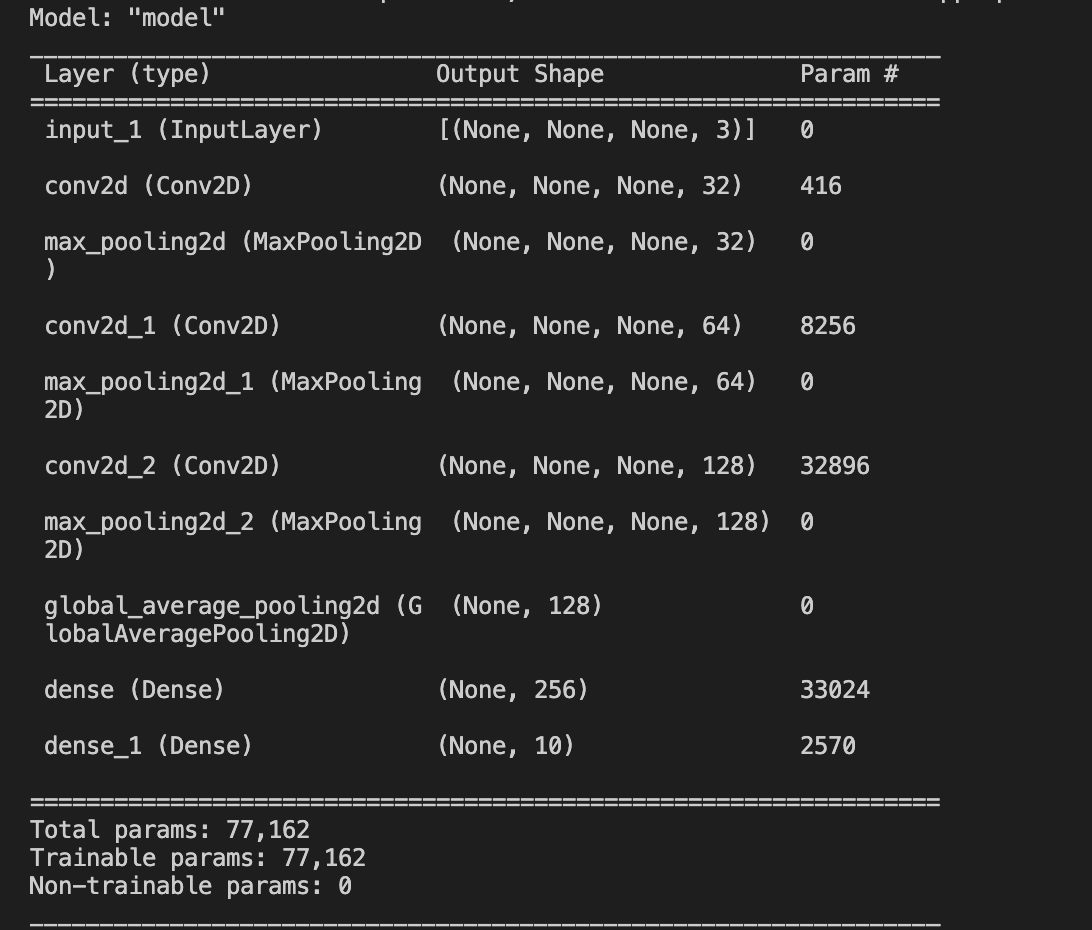
\includegraphics[scale=.4]{model_1_params.png} 
\caption{Model 1 Parameters}
\end{figure}

\begin{figure}
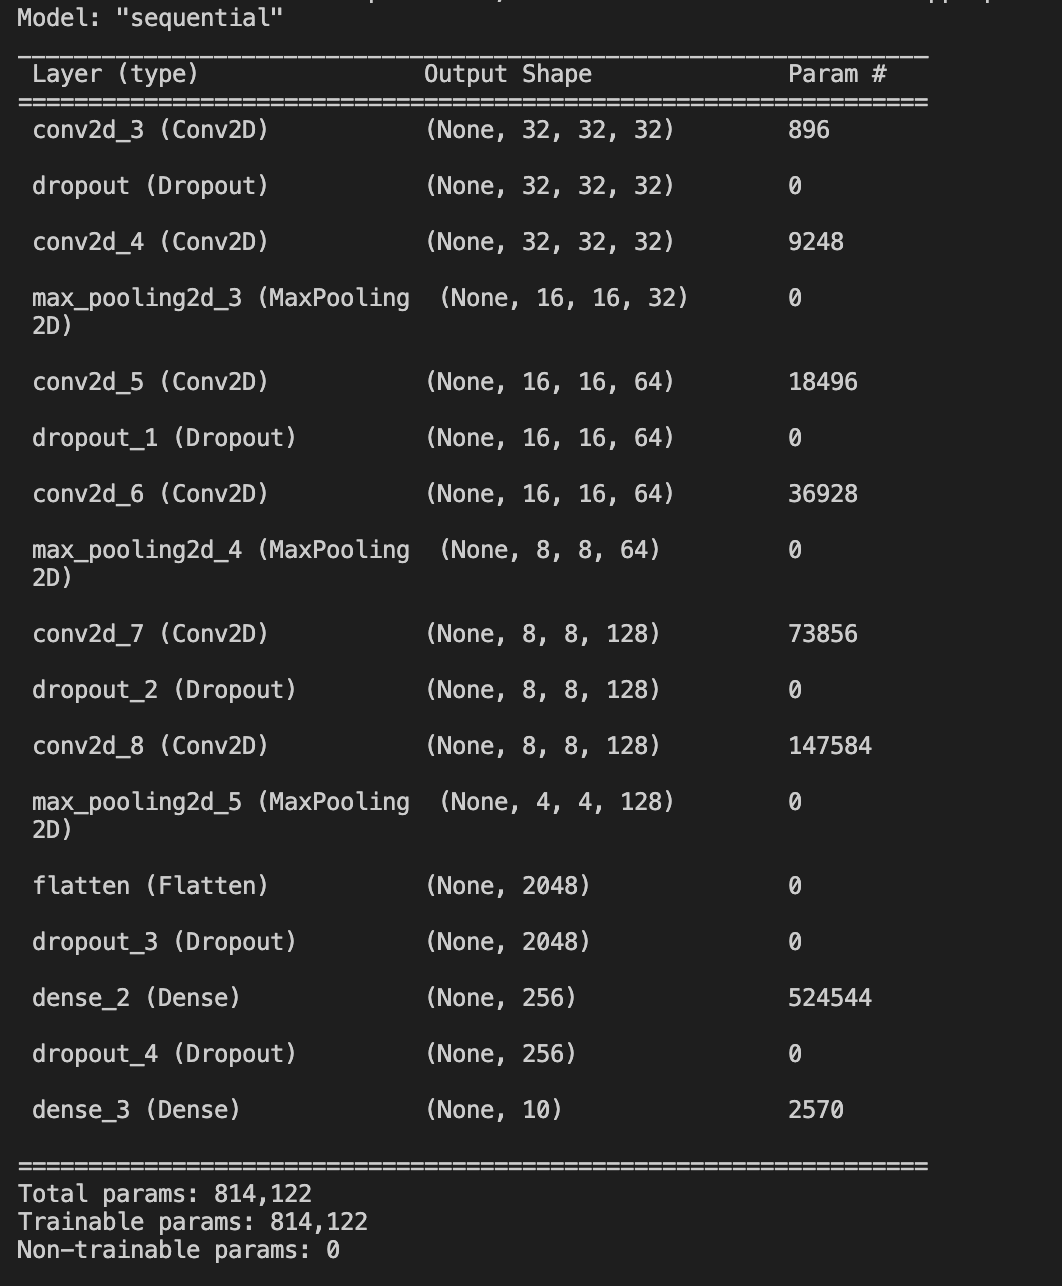
\includegraphics[scale=.4]{model_2_params.png} 
\caption{Model 2 Parameters}
\end{figure}

\section{Future Work}

Now we will work on reducing the CIFAR dataset efficiently. Then we will focus on tweaking the hyper-parameters for efficiency and recording the data


\end{document}